% Options for packages loaded elsewhere
\PassOptionsToPackage{unicode}{hyperref}
\PassOptionsToPackage{hyphens}{url}
%
\documentclass[
  ignorenonframetext,
]{beamer}
\usepackage{pgfpages}
\setbeamertemplate{caption}[numbered]
\setbeamertemplate{caption label separator}{: }
\setbeamercolor{caption name}{fg=normal text.fg}
\beamertemplatenavigationsymbolsempty
% Prevent slide breaks in the middle of a paragraph
\widowpenalties 1 10000
\raggedbottom
\setbeamertemplate{part page}{
  \centering
  \begin{beamercolorbox}[sep=16pt,center]{part title}
    \usebeamerfont{part title}\insertpart\par
  \end{beamercolorbox}
}
\setbeamertemplate{section page}{
  \centering
  \begin{beamercolorbox}[sep=12pt,center]{part title}
    \usebeamerfont{section title}\insertsection\par
  \end{beamercolorbox}
}
\setbeamertemplate{subsection page}{
  \centering
  \begin{beamercolorbox}[sep=8pt,center]{part title}
    \usebeamerfont{subsection title}\insertsubsection\par
  \end{beamercolorbox}
}
\AtBeginPart{
  \frame{\partpage}
}
\AtBeginSection{
  \ifbibliography
  \else
    \frame{\sectionpage}
  \fi
}
\AtBeginSubsection{
  \frame{\subsectionpage}
}

\usepackage{amsmath,amssymb}
\usepackage{lmodern}
\usepackage{iftex}
\ifPDFTeX
  \usepackage[T1]{fontenc}
  \usepackage[utf8]{inputenc}
  \usepackage{textcomp} % provide euro and other symbols
\else % if luatex or xetex
  \usepackage{unicode-math}
  \defaultfontfeatures{Scale=MatchLowercase}
  \defaultfontfeatures[\rmfamily]{Ligatures=TeX,Scale=1}
\fi
\usetheme[]{moon}
% Use upquote if available, for straight quotes in verbatim environments
\IfFileExists{upquote.sty}{\usepackage{upquote}}{}
\IfFileExists{microtype.sty}{% use microtype if available
  \usepackage[]{microtype}
  \UseMicrotypeSet[protrusion]{basicmath} % disable protrusion for tt fonts
}{}
\makeatletter
\@ifundefined{KOMAClassName}{% if non-KOMA class
  \IfFileExists{parskip.sty}{%
    \usepackage{parskip}
  }{% else
    \setlength{\parindent}{0pt}
    \setlength{\parskip}{6pt plus 2pt minus 1pt}}
}{% if KOMA class
  \KOMAoptions{parskip=half}}
\makeatother
\usepackage{xcolor}
\newif\ifbibliography
\setlength{\emergencystretch}{3em} % prevent overfull lines
\setcounter{secnumdepth}{-\maxdimen} % remove section numbering


\providecommand{\tightlist}{%
  \setlength{\itemsep}{0pt}\setlength{\parskip}{0pt}}\usepackage{longtable,booktabs,array}
\usepackage{calc} % for calculating minipage widths
\usepackage{caption}
% Make caption package work with longtable
\makeatletter
\def\fnum@table{\tablename~\thetable}
\makeatother
\usepackage{graphicx}
\makeatletter
\def\maxwidth{\ifdim\Gin@nat@width>\linewidth\linewidth\else\Gin@nat@width\fi}
\def\maxheight{\ifdim\Gin@nat@height>\textheight\textheight\else\Gin@nat@height\fi}
\makeatother
% Scale images if necessary, so that they will not overflow the page
% margins by default, and it is still possible to overwrite the defaults
% using explicit options in \includegraphics[width, height, ...]{}
\setkeys{Gin}{width=\maxwidth,height=\maxheight,keepaspectratio}
% Set default figure placement to htbp
\makeatletter
\def\fps@figure{htbp}
\makeatother

\makeatletter
\@ifpackageloaded{tcolorbox}{}{\usepackage[many]{tcolorbox}}
\@ifpackageloaded{fontawesome5}{}{\usepackage{fontawesome5}}
\definecolor{quarto-callout-color}{HTML}{909090}
\definecolor{quarto-callout-note-color}{HTML}{0758E5}
\definecolor{quarto-callout-important-color}{HTML}{CC1914}
\definecolor{quarto-callout-warning-color}{HTML}{EB9113}
\definecolor{quarto-callout-tip-color}{HTML}{00A047}
\definecolor{quarto-callout-caution-color}{HTML}{FC5300}
\definecolor{quarto-callout-color-frame}{HTML}{acacac}
\definecolor{quarto-callout-note-color-frame}{HTML}{4582ec}
\definecolor{quarto-callout-important-color-frame}{HTML}{d9534f}
\definecolor{quarto-callout-warning-color-frame}{HTML}{f0ad4e}
\definecolor{quarto-callout-tip-color-frame}{HTML}{02b875}
\definecolor{quarto-callout-caution-color-frame}{HTML}{fd7e14}
\makeatother
\makeatletter
\makeatother
\makeatletter
\makeatother
\makeatletter
\@ifpackageloaded{caption}{}{\usepackage{caption}}
\AtBeginDocument{%
\ifdefined\contentsname
  \renewcommand*\contentsname{Table of contents}
\else
  \newcommand\contentsname{Table of contents}
\fi
\ifdefined\listfigurename
  \renewcommand*\listfigurename{List of Figures}
\else
  \newcommand\listfigurename{List of Figures}
\fi
\ifdefined\listtablename
  \renewcommand*\listtablename{List of Tables}
\else
  \newcommand\listtablename{List of Tables}
\fi
\ifdefined\figurename
  \renewcommand*\figurename{Figure}
\else
  \newcommand\figurename{Figure}
\fi
\ifdefined\tablename
  \renewcommand*\tablename{Table}
\else
  \newcommand\tablename{Table}
\fi
}
\@ifpackageloaded{float}{}{\usepackage{float}}
\floatstyle{ruled}
\@ifundefined{c@chapter}{\newfloat{codelisting}{h}{lop}}{\newfloat{codelisting}{h}{lop}[chapter]}
\floatname{codelisting}{Listing}
\newcommand*\listoflistings{\listof{codelisting}{List of Listings}}
\makeatother
\makeatletter
\@ifpackageloaded{caption}{}{\usepackage{caption}}
\@ifpackageloaded{subcaption}{}{\usepackage{subcaption}}
\makeatother
\makeatletter
\@ifpackageloaded{tcolorbox}{}{\usepackage[many]{tcolorbox}}
\makeatother
\makeatletter
\@ifundefined{shadecolor}{\definecolor{shadecolor}{rgb}{.97, .97, .97}}
\makeatother
\makeatletter
\makeatother
\ifLuaTeX
  \usepackage{selnolig}  % disable illegal ligatures
\fi
\IfFileExists{bookmark.sty}{\usepackage{bookmark}}{\usepackage{hyperref}}
\IfFileExists{xurl.sty}{\usepackage{xurl}}{} % add URL line breaks if available
\urlstyle{same} % disable monospaced font for URLs
\hypersetup{
  pdftitle={Introduction to Medical Statistics},
  pdfauthor={Anna-Bettina Haidich Konstantinos Bougioukas Medical Statistics October 10, 2022},
  hidelinks,
  pdfcreator={LaTeX via pandoc}}

\title{Introduction to Medical Statistics}
\author{Anna-Bettina HaidichKonstantinos BougioukasMedical
StatisticsOctober 10, 2022}
\date{}

\begin{document}
\frame{\titlepage}
\ifdefined\Shaded\renewenvironment{Shaded}{\begin{tcolorbox}[sharp corners, interior hidden, boxrule=0pt, borderline west={3pt}{0pt}{shadecolor}, frame hidden, enhanced, breakable]}{\end{tcolorbox}}\fi

\begin{frame}{Online textbook of the course}
\protect\hypertarget{online-textbook-of-the-course}{}
The online textbook includes two Parts, ``Medical Statistics'' and
``Jamovi LAB''. For each theoretical chapter (e.g.,
\href{https://bougioukas-medstatsjamovi.netlify.app/introduction.html}{``Introduction''}.
) in first part there is a practical lab with Jamovi in the second part
(e.g.,
\href{https://bougioukas-medstatsjamovi.netlify.app/lab1.html}{``Lab
I:Introduction to Jamovi''}.

\begin{figure}

\hfill{} 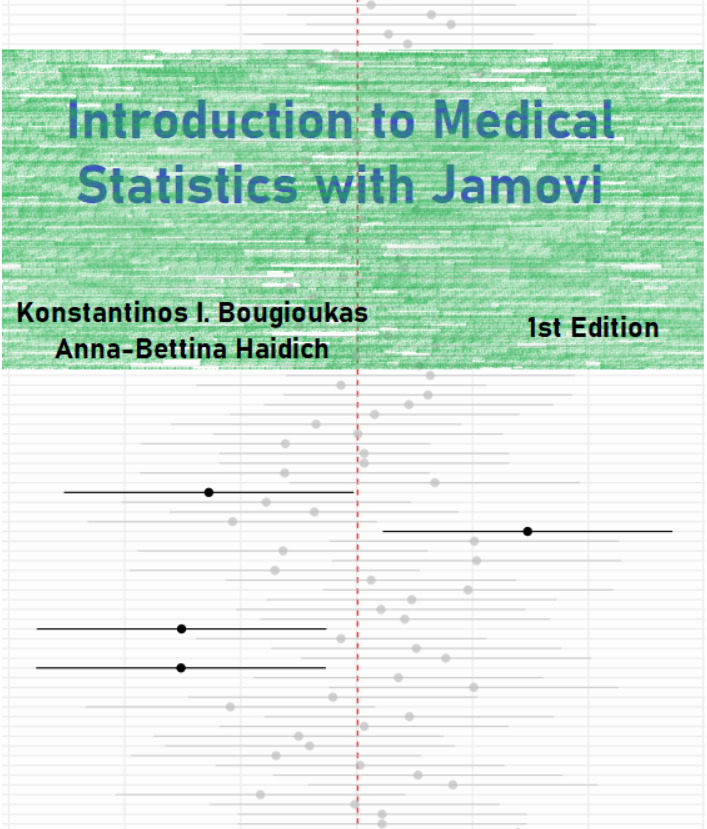
\includegraphics{images_slides/cover2.png}

\end{figure}
\end{frame}

\begin{frame}{Objectives of this lecture}
\protect\hypertarget{objectives-of-this-lecture}{}
\begin{itemize}
\item
  Distinguish descriptive from inferential statistics.
\item
  Explain the difference between qualitative and quantitative data.
\item
  Understand the difference between dependent and independent variables.
\item
  Identify the type of any given variable
  (nominal/ordinal/discrete/contnuous).
\end{itemize}
\end{frame}

\begin{frame}{Main branches of Statistics}
\protect\hypertarget{main-branches-of-statistics}{}
\begin{columns}[T]
\begin{column}{0.7\textwidth}
\begin{figure}

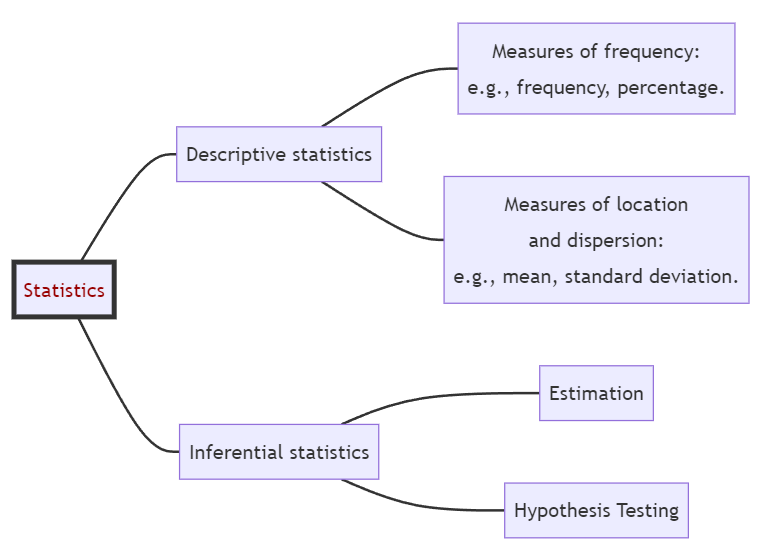
\includegraphics[width=0.9\textwidth,height=\textheight]{images_slides/branches3.png} \hfill{}

\end{figure}
\end{column}

\begin{column}{0.3\textwidth}
Statistics is an empirical method for collecting, organizing,
summarizing, and presenting data, and for making inferences about the
population from which the data are drawn.

\begin{itemize}
\item
  Descriptive statistics aim at {summarizing} large quantities of data
  by a few numbers.
\item
  Inferential statistics aim at {generalizing} observations made on a
  sample to a whole population.
\end{itemize}
\end{column}
\end{columns}
\end{frame}

\begin{frame}{Biomedical Data}
\protect\hypertarget{biomedical-data}{}
The data may include:

\begin{itemize}
\tightlist
\item
  {administrative} health data (data generated through the routine
  administration of healthcare programs)
\item
  {biomarker} data (e.g., metabolomics)
\item
  {biometric} data (e.g., data from wearable technologies)
\item
  {images} etc.
\end{itemize}

These data may originate from many different sources, including
{electronic health records (EHRs), clinical registries, biobanks, the
internet and patient self-reports}.
\end{frame}

\begin{frame}{From Data to Knowledge}
\protect\hypertarget{from-data-to-knowledge}{}
Biomedical data can be transformed into {information}. This information
can become {knowledge} if the researchers and clinicians understand it.

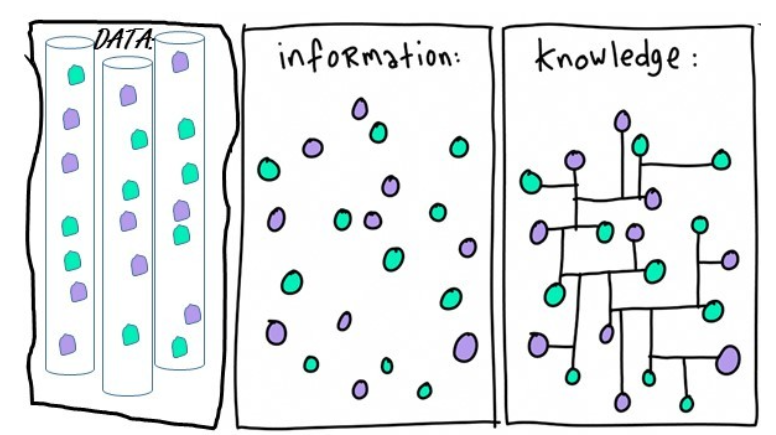
\includegraphics{images_slides/info.png}
\end{frame}

\begin{frame}{Data structures}
\protect\hypertarget{data-structures}{}
There are three main data structures:

\begin{itemize}
\item
  {Structured} data is generally tabular data that is represented by
  {columns} and {rows} in a database.
\item
  {Semi-Structured} data is a form of structured data that does not obey
  the tabular structure, yet does have some structural properties (e.g.,
  emails).
\item
  {Unstructured} data usually open text (such as social media posts),
  images, videos, etc., that have {no predetermined organization or
  design}.
\end{itemize}

\begin{figure}

{\centering 
\includegraphics{images_slides/tweet.png}

}

\end{figure}

In this course we use data organized in a {structured format
(spreadsheets)}. In statistics, tabular data refers to data that are
organized in a table with rows and columns. A {row} is a observation (or
record), which corresponds to the statistical unit of the dataset. The
{columns} are the variables (or characteristics) of interest.
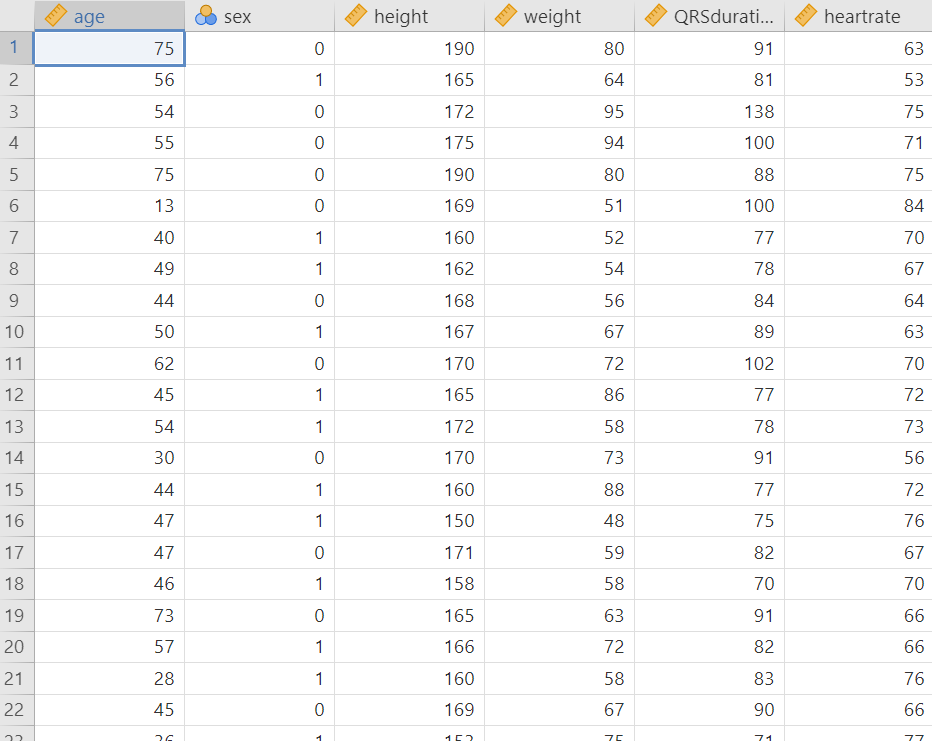
\includegraphics{images_slides/dat.png}
\end{frame}

\begin{frame}{Variables}
\protect\hypertarget{variables}{}
\begin{tcolorbox}[enhanced jigsaw, colframe=quarto-callout-tip-color-frame, colback=white, rightrule=.15mm, opacitybacktitle=0.6, opacityback=0, toprule=.15mm, breakable, colbacktitle=quarto-callout-tip-color!10!white, bottomtitle=1mm, bottomrule=.15mm, title={Variable}, left=2mm, toptitle=1mm, titlerule=0mm, coltitle=black, arc=.35mm, leftrule=.75mm]
A {variable} is a quantity or property that is free to vary, or take on
different values. To gain information on a variable, it is necessary to
design and conduct experiments.
\end{tcolorbox}

\begin{itemize}[<+->]
\item
  An {independent} variable is the variable that is {changed} or
  {controlled} in a scientific experiment to test the effects on another
  variable.
\item
  A {dependent (outcome)} variable is {the variable being tested} in a
  scientific experiment and is affected by at least one independent
  variable.
\end{itemize}
\end{frame}

\begin{frame}{Example 1}
\protect\hypertarget{example-1}{}
Suppose an investigator is examining whether hepatitis B antigen affects
liver function test results.

\begin{itemize}[<+->]
\item
  {\textbf{Independent variable}} of interest: the presence or absence
  of the hepatitis B antigen
\item
  {\textbf{Dependent variable}}: the liver function test result, as it
  is affected by hepatitis B antigen.
\end{itemize}
\end{frame}

\begin{frame}{Example 2}
\protect\hypertarget{example-2}{}
An investigator is studying the effectiveness of a newly developed
medicine to treat constipation. The treatment group receives the new
medication and the control group receives a placebo. The investigator
measures the number of days between taking the drug and the first bowel
movement among participants in both control and treatment groups.

\begin{itemize}
\item
  {\textbf{Independent variable}} of interest: the group
  assignment---treatment or control---is the independent variable
  because it is manipulated by the investigator and it affects the
  length of time until the first bowel movement.
\item
  {\textbf{Dependent variable}}: the number of days until the first
  bowel movement is the dependent variable because it is affected by the
  group assignment or whether the participant received the new drug or
  the placebo.
\end{itemize}
\end{frame}

\begin{frame}{Types of Data in Variables}
\protect\hypertarget{types-of-data-in-variables}{}
Data in variable can be either {categorical} or {numerical} (otherwise
known as qualitative and quantitative) in nature:

\begin{figure}

{\centering 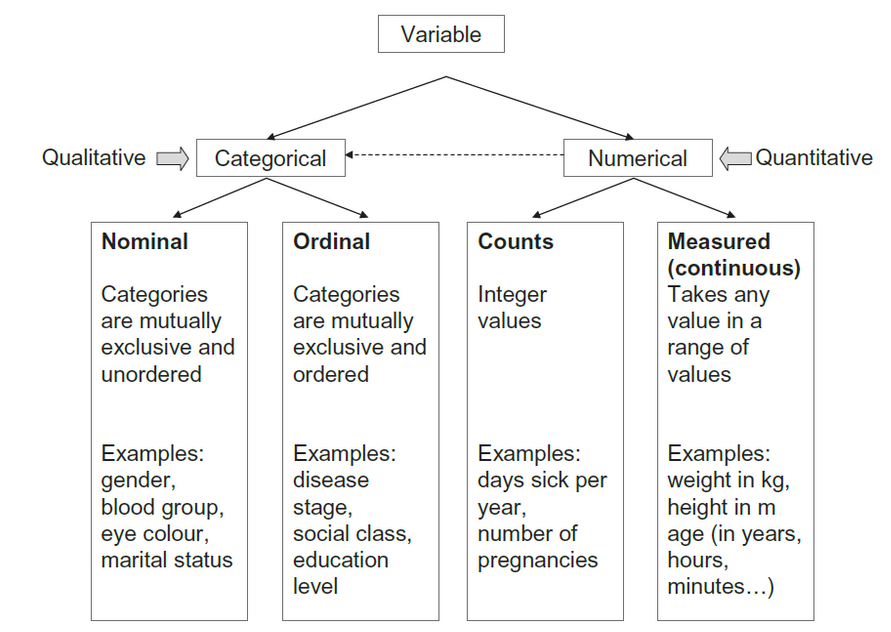
\includegraphics{images_slides/types.png}

}

\end{figure}
\end{frame}

\begin{frame}{Categorical Data}
\protect\hypertarget{categorical-data}{}
{\textbf{A. Nominal Data}}

Nominal categorical data are data that one can name and put into
categories. They are not measured but simply counted. They often consist
of \textbf{unordered} observations which have two categories and are
often know as \textbf{binary}. For example: {dead or alive; cured or not
cured; pregnant or not pregnant}.

However, nominal categorical data often can have \textbf{more than two
categories}, for example, {blood group A, B, AB, O; country of origin;
ethnic group; eye color}.

\begin{tcolorbox}[enhanced jigsaw, colframe=quarto-callout-important-color-frame, colback=white, rightrule=.15mm, opacitybacktitle=0.6, opacityback=0, toprule=.15mm, breakable, colbacktitle=quarto-callout-important-color!10!white, bottomtitle=1mm, bottomrule=.15mm, title=\textcolor{quarto-callout-important-color}{\faExclamation}\hspace{0.5em}{Numerical representation of categories are just codes}, left=2mm, toptitle=1mm, titlerule=0mm, coltitle=black, arc=.35mm, leftrule=.75mm]
We can denote a male and female as 1 and 2 for gender and denote A, B,
AB and O, as 1, 2, 3, and 4 for blood type. Unlike numerical data, the
numbers representing different categories \textbf{do not have
mathematical meaning} (they are just codes).
\end{tcolorbox}

{\textbf{Β. Ordinal Data}}

If there are more than two categories of classification it may be
possible to \textbf{order} them in some way. For example, {after
treatment a patient may be either improved, the same or worse}.

Another example of an ordinal variable is the variable {pain} where a
subject is asked to describe the pain verbally as {minimal, moderate,
severe, or unbearable}.

\begin{tcolorbox}[enhanced jigsaw, colframe=quarto-callout-important-color-frame, colback=white, rightrule=.15mm, opacitybacktitle=0.6, opacityback=0, toprule=.15mm, breakable, colbacktitle=quarto-callout-important-color!10!white, bottomtitle=1mm, bottomrule=.15mm, title=\textcolor{quarto-callout-important-color}{\faExclamation}\hspace{0.5em}{Collapsion of categories leads to a loss of information}, left=2mm, toptitle=1mm, titlerule=0mm, coltitle=black, arc=.35mm, leftrule=.75mm]
Ordinal data are often reduced to two categories to simplify analysis
and presentation, which may result in a \textbf{considerable loss of
information}.
\end{tcolorbox}
\end{frame}

\begin{frame}{Numerical Data}
\protect\hypertarget{numerical-data}{}
{\textbf{A. Discrete (or count) Data}}

Counts can only be a whole number or integer value, for example, {the
number of children: 0, 1, 2, 3, etc}.

Other examples are often {counts per unit of time} such as the number of
deaths in a hospital per year, the number of visits to the GP in a year,
or the number of attacks of asthma a person has per month.

The difference between discrete data and the ordinal data can be seen by
considering an example of each:

\begin{tcolorbox}[enhanced jigsaw, colframe=quarto-callout-note-color-frame, colback=white, rightrule=.15mm, opacitybacktitle=0.6, opacityback=0, toprule=.15mm, breakable, colbacktitle=quarto-callout-note-color!10!white, bottomtitle=1mm, bottomrule=.15mm, title={\textbf{Example: Ordinal Vs Discrete data}}, left=2mm, toptitle=1mm, titlerule=0mm, coltitle=black, arc=.35mm, leftrule=.75mm]
\textbf{\emph{Ordinal categorical:}} Stage of breast cancer: I II III IV

\textbf{\emph{Discrete numerical:}} Number of children: 0 1 2 3 4 5+

We \textbf{cannot} say that stage IV is twice as bad as stage II nor
that the difference between stages I and II is equivalent to that
between stages III and IV. In contrast, three children are three times
as many as one, and a difference of one means the same throughout the
range of values.
\end{tcolorbox}

{\textbf{Β. Continuous (or measured) Data}}

Continuous data are measurements with units that can, in theory at
least, {take any value within a given range} (they are restricted by the
accuracy of the measuring instrument). These data contain the most
information, and are the ones most commonly used in statistics. Examples
of continuous data are {age, weight, height, SBP, temperature}.

\begin{tcolorbox}[enhanced jigsaw, colframe=quarto-callout-important-color-frame, colback=white, rightrule=.15mm, opacitybacktitle=0.6, opacityback=0, toprule=.15mm, breakable, colbacktitle=quarto-callout-important-color!10!white, bottomtitle=1mm, bottomrule=.15mm, title=\textcolor{quarto-callout-important-color}{\faExclamation}\hspace{0.5em}{Categorization of numerical data leads to a loss of information}, left=2mm, toptitle=1mm, titlerule=0mm, coltitle=black, arc=.35mm, leftrule=.75mm]

For simplicity, it is often the case in medicine that continuous data
are dichotomized to make nominal data. For example, the diastolic blood
pressure (DBP), which is continuous, is converted into hypertension
(\textgreater90 mmHg) and normotension (≤90 mmHg). There are \textbf{two
main reasons} for doing this:

\begin{enumerate}
[(a)]
\item
  It is easier to \textbf{describe a population by the proportion} of
  people affected, for example, the proportion of people in the
  population with hypertension is 10\%.
\item
  It helps to \textbf{make a decision}: if a person has hypertension,
  then they will get treatment, and this is easier if high blood
  pressure has been categorized.
\end{enumerate}

\end{tcolorbox}
\end{frame}

\begin{frame}{Question 1}
\protect\hypertarget{question-1}{}
Which are the main branches of statistics?

\begin{itemize}[<+->]
\tightlist
\item
  {The two branches of statistics are descriptive statistics and
  inferential statistics.}
\end{itemize}
\end{frame}

\begin{frame}{Question 2}
\protect\hypertarget{question-2}{}
What is the difference between dependent and independent variables?

\begin{itemize}[<+->]
\tightlist
\item
  {A dependent variable is the variable being tested and measured in a
  scientific experiment (outcome). An independent variable is the
  variable that is changed or controlled in a scientific experiment to
  test the effects on the dependent variable.}
\end{itemize}
\end{frame}

\begin{frame}{Question 3}
\protect\hypertarget{question-3}{}
Try to identify the independent and dependent variables in the following
example study:

``Examining the difference between paracetamol and aspirin in the relief
of pain experienced by migraine sufferers.''

\begin{itemize}[<+->]
\tightlist
\item
  {Independent variable is the type of therapy (paracetamol or aspirin)
  and dependent variable is measured experience of pain relief.}
\end{itemize}
\end{frame}

\begin{frame}{Question 4}
\protect\hypertarget{question-4}{}
Which of the following is a qualitative nominal variable:

\begin{enumerate}
[a.]
\tightlist
\item
  Value of blood pH
\item
  Sensitivity of a diagnostic test (poor, moderate, high)
\item
  Hospitalization expenses in a hospital
\item
  Assignment of a person in one of three groups in a clinical trial
\end{enumerate}

\begin{itemize}[<+->]
\tightlist
\item
  {\textbf{d.} Assignment of a person in one of three groups in a
  clinical trial}
\end{itemize}
\end{frame}

\begin{frame}{Question 5}
\protect\hypertarget{question-5}{}
Which of the following is a quantitative continuous variable:

\begin{enumerate}
[a.]
\tightlist
\item
  Number of doctors in a hospital
\item
  An individual's health status (healthy/diseased)
\item
  Blood cholesterol levels (mg/dL)
\item
  Result of a biopsy (positive/negative)
\end{enumerate}

\begin{itemize}[<+->]
\tightlist
\item
  {\textbf{c.} Blood cholesterol levels (mg/dL)}
\end{itemize}
\end{frame}

\begin{frame}{}
\protect\hypertarget{section}{}

\includegraphics{images_slides/thank.png}
\end{frame}



\end{document}
